\documentclass[tikz,border=2mm]{standalone}
\usetikzlibrary{shapes.geometric, arrows.meta, positioning, calc}

\begin{document}
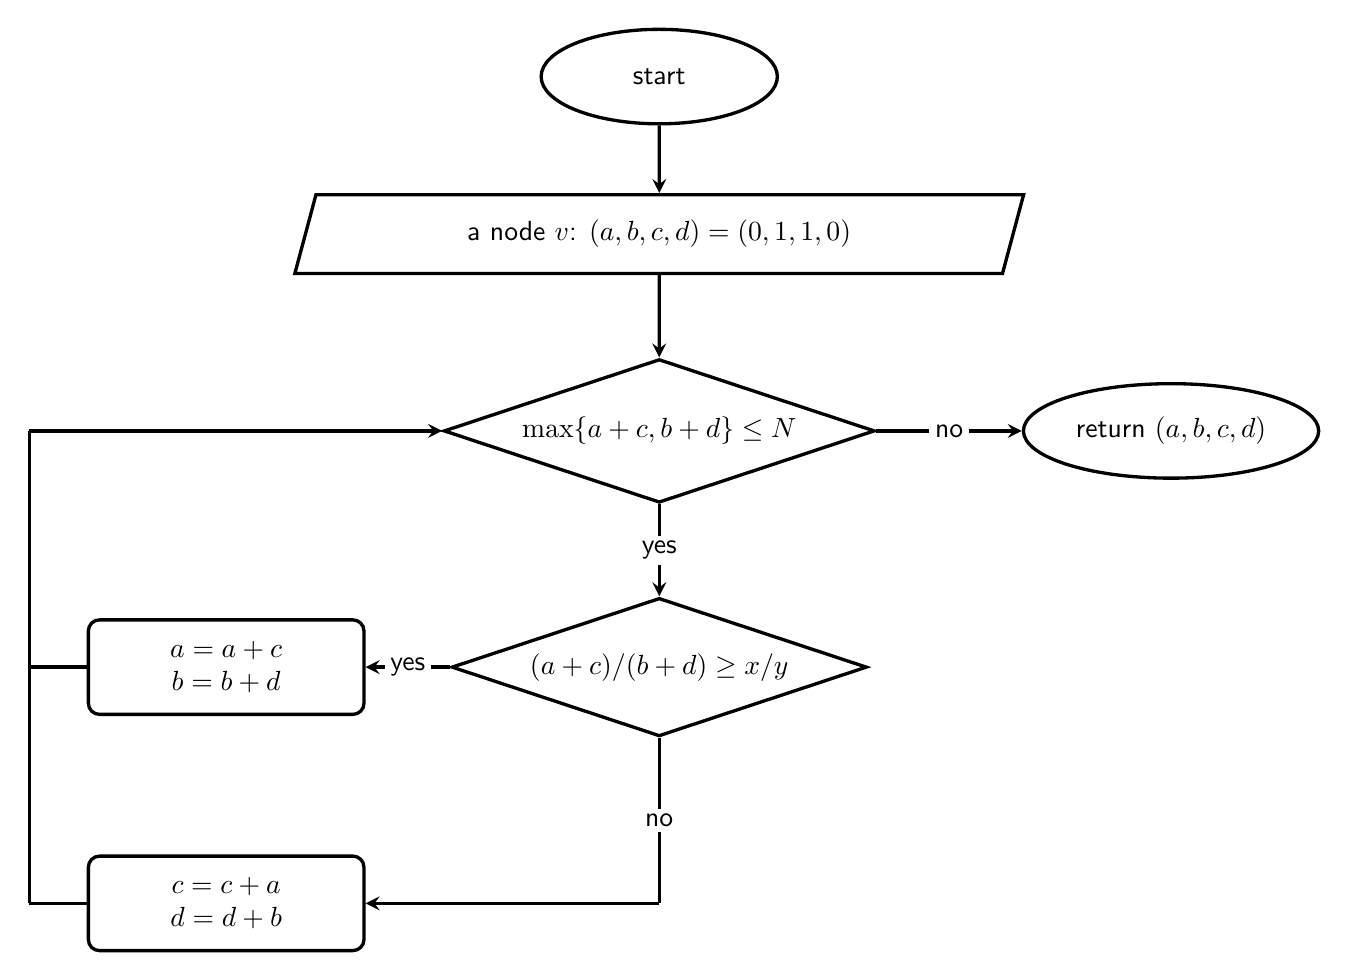
\begin{tikzpicture}[
    >=stealth,
    thick,
    startstop/.style={ellipse, draw, very thick, minimum width=3cm, minimum height=1.2cm, fill=white, align=center},
    io/.style={trapezium, trapezium left angle=75, trapezium right angle=105, draw, very thick, minimum width=5cm, minimum height=1cm, fill=white, align=center},
    decision/.style={diamond, draw, very thick, minimum width=5cm, minimum height=1.5cm, aspect=3, fill=white, align=center},
    process/.style={rectangle, rounded corners, draw, very thick, minimum width=3.5cm, minimum height=1.2cm, fill=white, align=center},
    font=\sffamily
]

\node[startstop] (start) at (0, 0) {start};
\node[io] (init) at (0, -2) {a node $v$: $(a, b, c, d)=(0, 1, 1, 0)$};
\node[decision] (cond1) at (0, -4.5) {$\max\{a+c, b+d\}\le N$};
\node[startstop] (return) at (6.5, -4.5) {return $(a, b, c, d)$};
\node[decision] (cond2) at (0, -7.5) {$(a+c)/(b+d) \ge x/y$};
\node[process] (procyes) at (-5.5, -7.5) {$a = a + c$ \\ $b = b + d$};
\node[process] (procno) at (-5.5, -10.5) {$c = c + a$ \\ $d = d + b$};

\draw[->, very thick] (start) -- (init);
\draw[->, very thick] (init) -- (cond1);
\draw[->, very thick] (cond1.east) -- node[midway, fill=white, inner sep=2pt] {no} (return.west);
\draw[->, very thick] (cond1.south) -- node[midway, fill=white, inner sep=2pt] {yes} (cond2.north);
\draw[->, very thick] (cond2.west) -- node[midway, fill=white, inner sep=2pt] {yes} (procyes.east);
\draw[very thick] (cond2.south) -- node[midway, fill=white, inner sep=2pt] {no} (0, -10.5);
\draw[->, very thick] (0, -10.5) -- (procno.east);

\draw[very thick] (procno.west) -- (-8, -10.5);
\draw[very thick] (procyes.west) -- (-8, -7.5);
\draw[very thick] (-8, -10.5) -- (-8, -4.5);
\draw[->, very thick] (-8, -4.5) -- (cond1.west);

\end{tikzpicture}
\end{document}
